%% LyX 2.3.6.1 created this file.  For more info, see http://www.lyx.org/.
%% Do not edit unless you really know what you are doing.
\documentclass[11pt,openany]{uhthesis}
\usepackage[latin9]{inputenc}
\setcounter{secnumdepth}{3}
\setcounter{tocdepth}{3}
\usepackage{float}
\usepackage{bm}
\usepackage{amsmath}
\usepackage{graphicx}
\usepackage{setspace}
\usepackage[numbers,sort&compress]{natbib}
\usepackage{nomencl}
% the following is useful when we have the old nomencl.sty package
\providecommand{\printnomenclature}{\printglossary}
\providecommand{\makenomenclature}{\makeglossary}
\makenomenclature
\onehalfspacing
\usepackage[unicode=true,pdfusetitle,
 bookmarks=true,bookmarksnumbered=false,bookmarksopen=false,
 breaklinks=false,pdfborder={0 0 1},backref=false,colorlinks=false]
 {hyperref}

\makeatletter

%%%%%%%%%%%%%%%%%%%%%%%%%%%%%% LyX specific LaTeX commands.
%% Because html converters don't know tabularnewline
\providecommand{\tabularnewline}{\\}

%%%%%%%%%%%%%%%%%%%%%%%%%%%%%% User specified LaTeX commands.
%!!!!!!!!!!!!!!!!!!!!!!!!!!!!!!!!!!!!!!!!!!!!!!!!!!!!!!!!!!!!!!!!!!!!!!!!!!!!!!
%!NOTE: This example file has been prepared according to the University of
%!      Hawaii Style & Policy Manual for Theses and Dissertations dated
%!      "Revised September 2010". If you have one with a later date, you may
%!      need to make revisions to this document as well. In any event, making
%!      sure your thesis complies with Graduate Education guidelines is
%!      ultimately your responsibility. Caveat LaTeXtor. :)
%!!!!!!!!!!!!!!!!!!!!!!!!!!!!!!!!!!!!!!!!!!!!!!!!!!!!!!!!!!!!!!!!!!!!!!!!!!!!!!

%% The options are (you can only choose one from each group):
%%
%% 10pt, 11pt, 12pt: chooses the point size for the document. "11pt" is the
%%                   default.
%%
%% oneside, twoside: whether you want your document onesided or twosided. Note
%%                   that twosided is not guaranteed to work, and style
%%                   guidelines prohibit double sided printouts on final
%%                   copy. "oneside" is the default.
%%
%% draft, final: when printing drafts you can save a lot of paper by using the
%%               "draft" option. It switches to single spacing, displays overful
%%               hboxes with a black box, prints a version number on title page 
%%               and omits signature page. Of course for the final copy make
%%               sure to use the "final" option! "final" is the default.
%%
%% thesis, dissertation: switches between the style for a master's thesis and a 
%%                       Ph.D. dissertation. The differences are fairly minor
%%                       and limited to the front matter. "thesis" is the
%%                       default.
%%
%% actual, proposal: switches between actual document and proposal mode. In
%%                   proposal mode: the title page is simplified and the
%%                   version number is always printed.
%%
%%% Load the new uhthesis document class


%%% Load some useful packages:
%% New LaTeX2e graphics support
%% Package to linebreak URLs in a sane manner.
\usepackage{graphicx}
\usepackage{amssymb}
\usepackage{url}
\usepackage[titletoc,title]{appendix}
\usepackage{emptypage}
\usepackage{lastpage} 
\usepackage{afterpage}

\versionnum{4.0.0}

%%% End of preamble

\makeatother

\usepackage{listings}
\def\eqdeclaration#1{, see equation\nobreakspace(#1)}
\def\pagedeclaration#1{, page\nobreakspace#1}
\def\nomname{Nomenclature}
\renewcommand{\lstlistingname}{Listing}

\begin{document}
\title{Computational Fluid Dynamics Simulations of Overflow Patterns in Utility-Chamber and Hydrodynamic Stresses in Vegetation Zone} 
\author{(FirstName MiddleName LastName)} 
\degreemonth{(Degree-AwardedMonth)} 
\degreeyear{(Degree-Awarded Year)} 
\degree{(Master of Science)} 
\chair{(Full Name)} 
\othermembers{
(Committee Member No 1 FullName)\\ 
(Committee Member No 2 FullName)\\  
(Committee Member No 3 FullName)
} 
\field{(Civil and Environmental Engineering)} 
\keywords{(keyword-1, keyword-2, keyword-3, ... )} 

\maketitle

\begin{frontmatter}

%%% Create the copyright page (optional)
\copyrightpage

%%% Bring in the dedication page from external file (optional)
\newpage

\begin{dedication} \null\vfil 
\begin{center}
{\large{}To my \_\_\_\_\_\_\_\_\_\_\_\_,}\\
{\large{}\vspace{12pt}
}{\large\par}
\par\end{center}

\begin{center}
{\large{}\_\_\_\_\_\_\_\_\_\_\_\_\_\_\_\_\_\_\_\_\_\_\_\_\_\_\_}{\large\par}
\par\end{center}

\vfil\null \end{dedication}

\pagebreak \null \newpage

\begin{acknowledgments}

Firstly, I want to express my appreciation and respect to my

\end{acknowledgments}

\pagebreak \null \newpage

\begin{abstract}
\begin{onehalfspace}
Lorem ipsum dolor sit amet, consectetur adipiscing elit, sed do eiusmod
tempor incididunt ut labore et dolore magna aliqua. Placerat vestibulum
lectus mauris ultrices eros in cursus turpis massa. Erat nam at lectus
urna duis convallis convallis tellus id. In fermentum posuere urna
nec tincidunt praesent semper feugiat nibh. Mattis rhoncus urna neque
viverra justo nec ultrices dui. A diam sollicitudin tempor id eu nisl.
Dictum fusce ut placerat orci nulla pellentesque dignissim enim sit.
Nisi vitae suscipit tellus mauris a diam maecenas. Proin libero nunc
consequat interdum varius sit amet mattis. Eu tincidunt tortor aliquam
nulla facilisi. Lorem sed risus ultricies tristique nulla aliquet.
Pharetra magna ac placerat vestibulum lectus. Odio aenean sed adipiscing
diam. Ullamcorper sit amet risus nullam eget felis eget nunc lobortis.
\end{onehalfspace}

Sodales ut eu sem integer vitae justo eget magna. Sagittis purus sit
amet volutpat. Sit amet dictum sit amet justo donec enim. Accumsan
in nisl nisi scelerisque eu ultrices. Purus viverra accumsan in nisl
nisi scelerisque eu. At tempor commodo ullamcorper a lacus vestibulum
sed arcu. Interdum velit laoreet id donec ultrices tincidunt arcu.
Nibh sit amet commodo nulla. Nibh sit amet commodo nulla facilisi
nullam vehicula. Ultrices dui sapien eget mi proin sed libero enim
sed. Donec et odio pellentesque diam. Lacus luctus accumsan tortor
posuere ac. Curabitur gravida arcu ac tortor dignissim convallis.
Amet porttitor eget dolor morbi non. Aliquam sem et tortor consequat
id porta nibh. Nulla facilisi morbi tempus iaculis urna id. Nisl suscipit
adipiscing bibendum est ultricies integer quis. Tincidunt dui ut ornare
lectus sit.

Aliquet risus feugiat in ante metus dictum. Posuere urna nec tincidunt
praesent semper feugiat nibh sed pulvinar. Neque gravida in fermentum
et sollicitudin ac. Pharetra pharetra massa massa ultricies mi. Ac
tincidunt vitae semper quis. Libero nunc consequat interdum varius
sit amet. Enim lobortis scelerisque fermentum dui faucibus in ornare
quam. Sed euismod nisi porta lorem mollis aliquam. Nisl suscipit adipiscing
bibendum est ultricies integer quis. Morbi enim nunc faucibus a pellentesque
sit amet. Justo eget magna fermentum iaculis eu non diam phasellus
vestibulum. A scelerisque purus semper eget duis at tellus.

Placerat in egestas erat imperdiet sed euismod nisi. Netus et malesuada
fames ac turpis egestas integer. Rutrum quisque non tellus orci ac
auctor augue mauris. Sed faucibus turpis in eu mi bibendum. Feugiat
nibh sed pulvinar proin. Nunc vel risus commodo viverra maecenas accumsan
lacus vel. A diam maecenas sed enim. Vel fringilla est ullamcorper
eget nulla. Massa vitae tortor condimentum lacinia quis. A condimentum
vitae sapien pellentesque habitant morbi tristique. Urna nec tincidunt
praesent semper feugiat nibh. Lectus vestibulum mattis ullamcorper
velit sed ullamcorper morbi tincidunt. Feugiat in fermentum posuere
urna nec tincidunt praesent semper. Dolor sit amet consectetur adipiscing
elit pellentesque habitant morbi tristique. Ipsum dolor sit amet consectetur
adipiscing elit pellentesque habitant. Pellentesque elit eget gravida
cum sociis natoque penatibus et magnis.
\end{abstract}

\pagebreak

\tableofcontents{}

\pagebreak

\listoftables

\pagebreak \null \newpage

\listoffigures

\pagebreak \null \newpage

\printnomenclature{}

\begin{onehalfspace}
\nomenclature[Z]{{$U$}}{flow speed} \nomenclature[C]{pHP}{\texttt{phaseHydrostaticPressure}}
\nomenclature[c]{pIOV}{\texttt{pressureInletOutletVelocity}} \nomenclature[C]{tIKEI}{\texttt{turbulentIntensityKineticEnergyInlet}}
\nomenclature[C]{tMLDRI}{\texttt{turbulentMixingLengthDissipationRateInlet}}
\nomenclature[C]{BC}{boundary condition} \nomenclature[C]{CFD}{computational fluid dynamics}
\nomenclature[Z]{$\bm{U}$}{flow vector} \nomenclature[Z]{${p}$}{pressure}
\nomenclature[Z]{$Q_\mathrm{in}$}{inflow rate [mgd] or [tons/s]}
\nomenclature[Z]{$f_\mathrm{b}$}{body force term} \nomenclature[Z]{$V_\mathrm{ic}$}{initial volume in chamber}
\nomenclature[Z]{${L}$}{chamber length} \nomenclature[Z]{${S}$}{inter-stem spacing}
\nomenclature[Z]{${T}$}{stress tensor} \nomenclature[Z]{${H}$}{chamber height}
\nomenclature[Z]{${h}$}{stem height} \nomenclature[Z]{${W}$}{chamber width}
\nomenclature[Z]{$D_\mathrm{o}$}{outlet diameter} \nomenclature[Z]{$D_\mathrm{s}$}{stem diameter}
\nomenclature[Z]{$D_\mathrm{i}$}{inlet diameter} \nomenclature[Z]{$n_\mathrm{x}$, $n_\mathrm{y}$,   $n_\mathrm{z}$}{mesh division numbers in $x$, $y$, and $z$ directions, respectively}
\nomenclature[G]{$\rho$}{density} \nomenclature[G]{$\theta$}{channel gradient}
\nomenclature[G]{$\tau$}{shear stress} \nomenclature[G]{$\alpha$}{fluid volume fraction}
\nomenclature[G]{$\lambda$}{stem occupancy fraction} \nomenclature[G]{$\nu$}{kinematic viscosity}
\nomenclature[G]{$\nu_t$}{turbulent kinematic viscosity} \nomenclature[Z]{$t_\mathrm{ss}$}{time to reach a steady state}
\nomenclature[Z]{$t_\mathrm{sm}$}{time occuring the first submerging of outlet pipe}
\nomenclature[Z]{$h_\mathrm{ss}$}{sewage level in a steady state}
\nomenclature[S]{$\mathrm{ic}$}{inside the chamber} \nomenclature[S]{$\mathrm{1}$}{water phase}
\nomenclature[S]{$\mathrm{0}$}{air phase} \nomenclature[S]{$\mathrm{b}$}{body}
\nomenclature[Z]{$\bm{m}$}{meter} \nomenclature[Z]{$\bm{mm}$}{millimeter}
\nomenclature[Z]{$\bm{cm}$}{centimeter} \nomenclature[Z]{$\bm{m/s}$}{meter per second}
\nomenclature[Z]{$\bm{ft}$}{foot} \nomenclature[Z]{$\bm{in}$}{inch}
\nomenclature[Z]{$\bm{ft/s}$}{foot per second} \nomenclature[Z]{$\bm{gal}$}{gallon}
\nomenclature[Z]{$\bm{s}$}{second} \nomenclature[Z]{$\bm{mgd}$}{million gallons per day}
\end{onehalfspace}

\pagebreak \newpage 

\end{frontmatter}

\clearpage{}

\chapter{Sewer Chamber Design under Critical Conditions using Computational
Fluid Dynamics (CFD)}

This chapter of the dissertation is a manuscript published in Desalination
and Water Treatment, 108 (2018) 1-14, doi: 10.5004/dwt.2018.22019.

Transient sewage flow patterns inside a utility chamber are ... 

\textit{Keywords: }Computational fluid dynamics (CFD); OpenFOAM; Sewer
design; manhole flow; urban runoff

\section{Introduction}

Lorem ipsum dolor sit amet, consectetur adipiscing elit, sed do eiusmod
tempor incididunt ut labore et dolore magna aliqua. Ante metus dictum
at tempor commodo. Quis risus sed vulputate odio ut enim. Sed elementum
tempus egestas sed. Nibh nisl condimentum id venenatis a\citep{Balogh-JoWEaIA-2012-10.1016_j.jweia.2012.02.023,Greifzu-EAoCFM-2016-10.1080_19942060.2015.1104266}.
Et egestas quis ipsum suspendisse ultrices gravida dictum fusce. Tempor
orci eu lobortis elementum nibh tellus molestie nunc. Feugiat pretium
nibh ipsum consequat. Posuere urna nec tincidunt praesent semper feugiat
nibh. Pellentesque dignissim enim sit amet venenatis. Amet purus gravida
quis blandit turpis cursus. Eu ultrices vitae auctor eu augue ut lectus
arcu bibendum. Habitant morbi tristique senectus et. Orci a scelerisque
purus semper eget duis. Elit scelerisque mauris pellentesque pulvinar
pellentesque. Turpis massa sed elementum tempus egestas sed. Eget
mi proin sed libero \citep{Kang-D-2017-10.1016_j.desal.2017.05.018,Kim-DaWT-2017:10.5004_dwt.2017.11423,Kim-DaWT-2017:10.5004_dwt.2017.11422}.
Tempor orci eu lobortis elementum nibh tellus molestie nunc. Feugiat
pretium nibh ipsum consequat. Posuere urna nec tincidunt praesent
semper feugiat nibh. Pellentesque dignissim enim sit amet venenatis.
Amet purus gravida quis blandit turpis cursus. Eu ultrices vitae auctor
eu augue ut lectus arcu bibendum. Habitant morbi tristique senectus
et. Orci a scelerisque purus se  \citep{AhrensGeveciEtAl-2005,Ayachit-2015}.

\section{Simulations}

\subsection{Governing equations}

A brief summary of governing equations is as follows. As noted above,
\texttt{interFoam} is a solver for two incompessible, isothermal,
immiscible fluid, which uses the volume of fluid (VOD) phase fraction.
The continuity and phase-fraction transport equations are 
\begin{equation}
\nabla\cdot\bm{U}=0
\end{equation}
and 
\begin{equation}
\frac{\partial\alpha_{1}}{\partial t}+\nabla\cdot\left(\bm{U}\alpha_{1}\right)=0
\end{equation}
respectively, and the momentum equation is 
\begin{equation}
\frac{\partial\left(\rho\bm{U}\right)}{\partial t}+\nabla\cdot\left(\rho\bm{U}\bm{U}\right)=-\nabla p+\nabla\cdot\bm{T}+\rho\bm{f}_{b}\label{eq:NS}
\end{equation}
where $\alpha_{1}$ is the phase-fraction of water, ranging from 0.0
to 1.0. In Eq. (\ref{eq:NS}), $\bm{T}$ in is the stress tensor and
$\bm{f}_{b}$ is a body force term including gravity and surface tension,
and the fluid density $\rho$ and viscosity $\mu$ are estimated as
\begin{align}
\rho & =\alpha_{1}\rho_{1}+\left(1-\alpha_{1}\right)\rho_{0}\\
\mu & =\alpha_{1}\mu_{1}+\left(1-\alpha_{1}\right)\mu_{0}
\end{align}
where the subscript 1 and 0 indicate water and air phases, respectively.
More details of the solver can be found elsewhere \citep{Weller-CiP-1998-10.1063_1.168744,Manual-OpenFOAMFoundation-2016}.

\subsection{Manhole structure and meshing}

Fig. \ref{fig:manhole-section-view} shows ... 

.

.

This is summarized in Table \ref{tab:dimensions}.

Fig. \ref{fig:mesh-struct} shows .. 

\section{Results and Discussions}

\subsection{Result section title }

Lorem ipsum dolor sit amet, consectetur adipiscing elit, sed do eiusmod
tempor incididunt ut labore et dolore magna aliqua. Morbi tristique
senectus et netus et malesuada. Fusce id velit ut tortor pretium.
Ac turpis egestas integer eget aliquet nibh praesent tristique. Odio
pellentesque diam volutpat commodo sed egestas egestas fringilla.
Maecenas ultricies mi eget mauris. Aliquam purus sit amet luctus.
Amet venenatis urna cursus eget. Turpis tincidunt id aliquet risus.
Eu augue ut lectus arcu bibendum at. Felis imperdiet proin fermentum
leo vel orci porta non. Morbi leo urna molestie at elementum eu. Risus
pretium quam vulputate dignissim suspendisse in est ante in. Nunc
non blandit massa enim. Turpis egestas sed tempus urna. 

\subsection{Tantalizing phenomena}

\subsubsection{3D investigation}

Lorem ipsum dolor sit amet, consectetur adipiscing elit, sed do eiusmod
tempor incididunt ut labore et dolore magna aliqua. Morbi tristique
senectus et netus et malesuada. Fusce id velit ut tortor pretium.
Ac turpis egestas integer eget aliquet nibh praesent tristique. Odio
pellentesque diam volutpat commodo sed egestas egestas fringilla.
Maecenas ultricies mi eget mauris. Aliquam purus sit amet luctus.
Amet venenatis urna cursus eget. Turpis tincidunt id aliquet risus.
Eu augue ut lectus arcu bibendum at. Felis imperdiet proin fermentum
leo vel orci porta non. Morbi leo urna molestie at elementum eu. Risus
pretium quam vulputate dignissim suspendisse in est ante in. Nunc
non blandit massa enim. Turpis egestas sed tempus urna 

\subsubsection{2D investigation}

\subsection{Result verification and convergence test}

In this section, we provide ...

\section{Conclusion}

In order to maintain ...

\paragraph{Acknowledgment}

This research used the Extreme Science and Engineering Discovery Environment
(XSEDE), which is supported by National Science Foundation grant number
ACI-1053575, and was financially supported by R. M. Towill Corporation,
Honolulu, Hawaii, USA. The authors appreciate Mr. Jonathan Imai for
his Solid Works drawing for the mesh generation.

\newpage\null
\vfill
\begin{table}[H]
\begin{centering}
\begin{tabular}{|l|r|r|r|r|}
\hline 
 & $D$ & $L$ & $W$ & $H$\tabularnewline
\hline 
\hline 
inlet pipe & 16.0 in. (0.406 m) & 16.0 ft (4.9 m) & -- & --\tabularnewline
\hline 
outlet pipe & 18.0 in. (0.457 m) & 22.0 ft (6.7 m) & -- & --\tabularnewline
\hline 
chamber & -- & 10.0 ft (3.0 m) & 4.0 ft (1.2 m) & 6.0 ft (1.8 m)\tabularnewline
\hline 
\end{tabular}
\par\end{centering}
\caption{Chamber and pipe dimensions. CFD simulations were conducted for three
outlet diameters: 18, 20, and 24 inches (0.457, 0.508, and 0.610 meters,
respectively).}

\label{tab:dimensions}
\end{table}

\vfill\newpage\null
\vfill
\begin{table}[H]
\begin{centering}
\begin{tabular}{|l|c|c|c|}
\hline 
 & water & air & unit\tabularnewline
\hline 
\hline 
fluid type & Newtonian & Newtonian & -\tabularnewline
\hline 
density, $\rho$ & 998.0 & 1.21 & kg/m\textsuperscript{3}\tabularnewline
\hline 
kinematic viscosity, $\nu$ & $1.0\times10^{-6}$ & $1.51\times10^{-5}$ & m\textsuperscript{2}/s\tabularnewline
\hline 
\end{tabular}
\par\end{centering}
\caption{Properties of water and air used for \texttt{interFoam} simulations.
In addition, the surface tension between water and air was set as
0.072 N/m and the gravitational acceleration (9.81m/s\protect\protect\textsuperscript{2})
was used.}

\label{tab:matt-prop}
\end{table}

\vfill\newpage\null
\vfill
\begin{figure}[H]
\begin{centering}
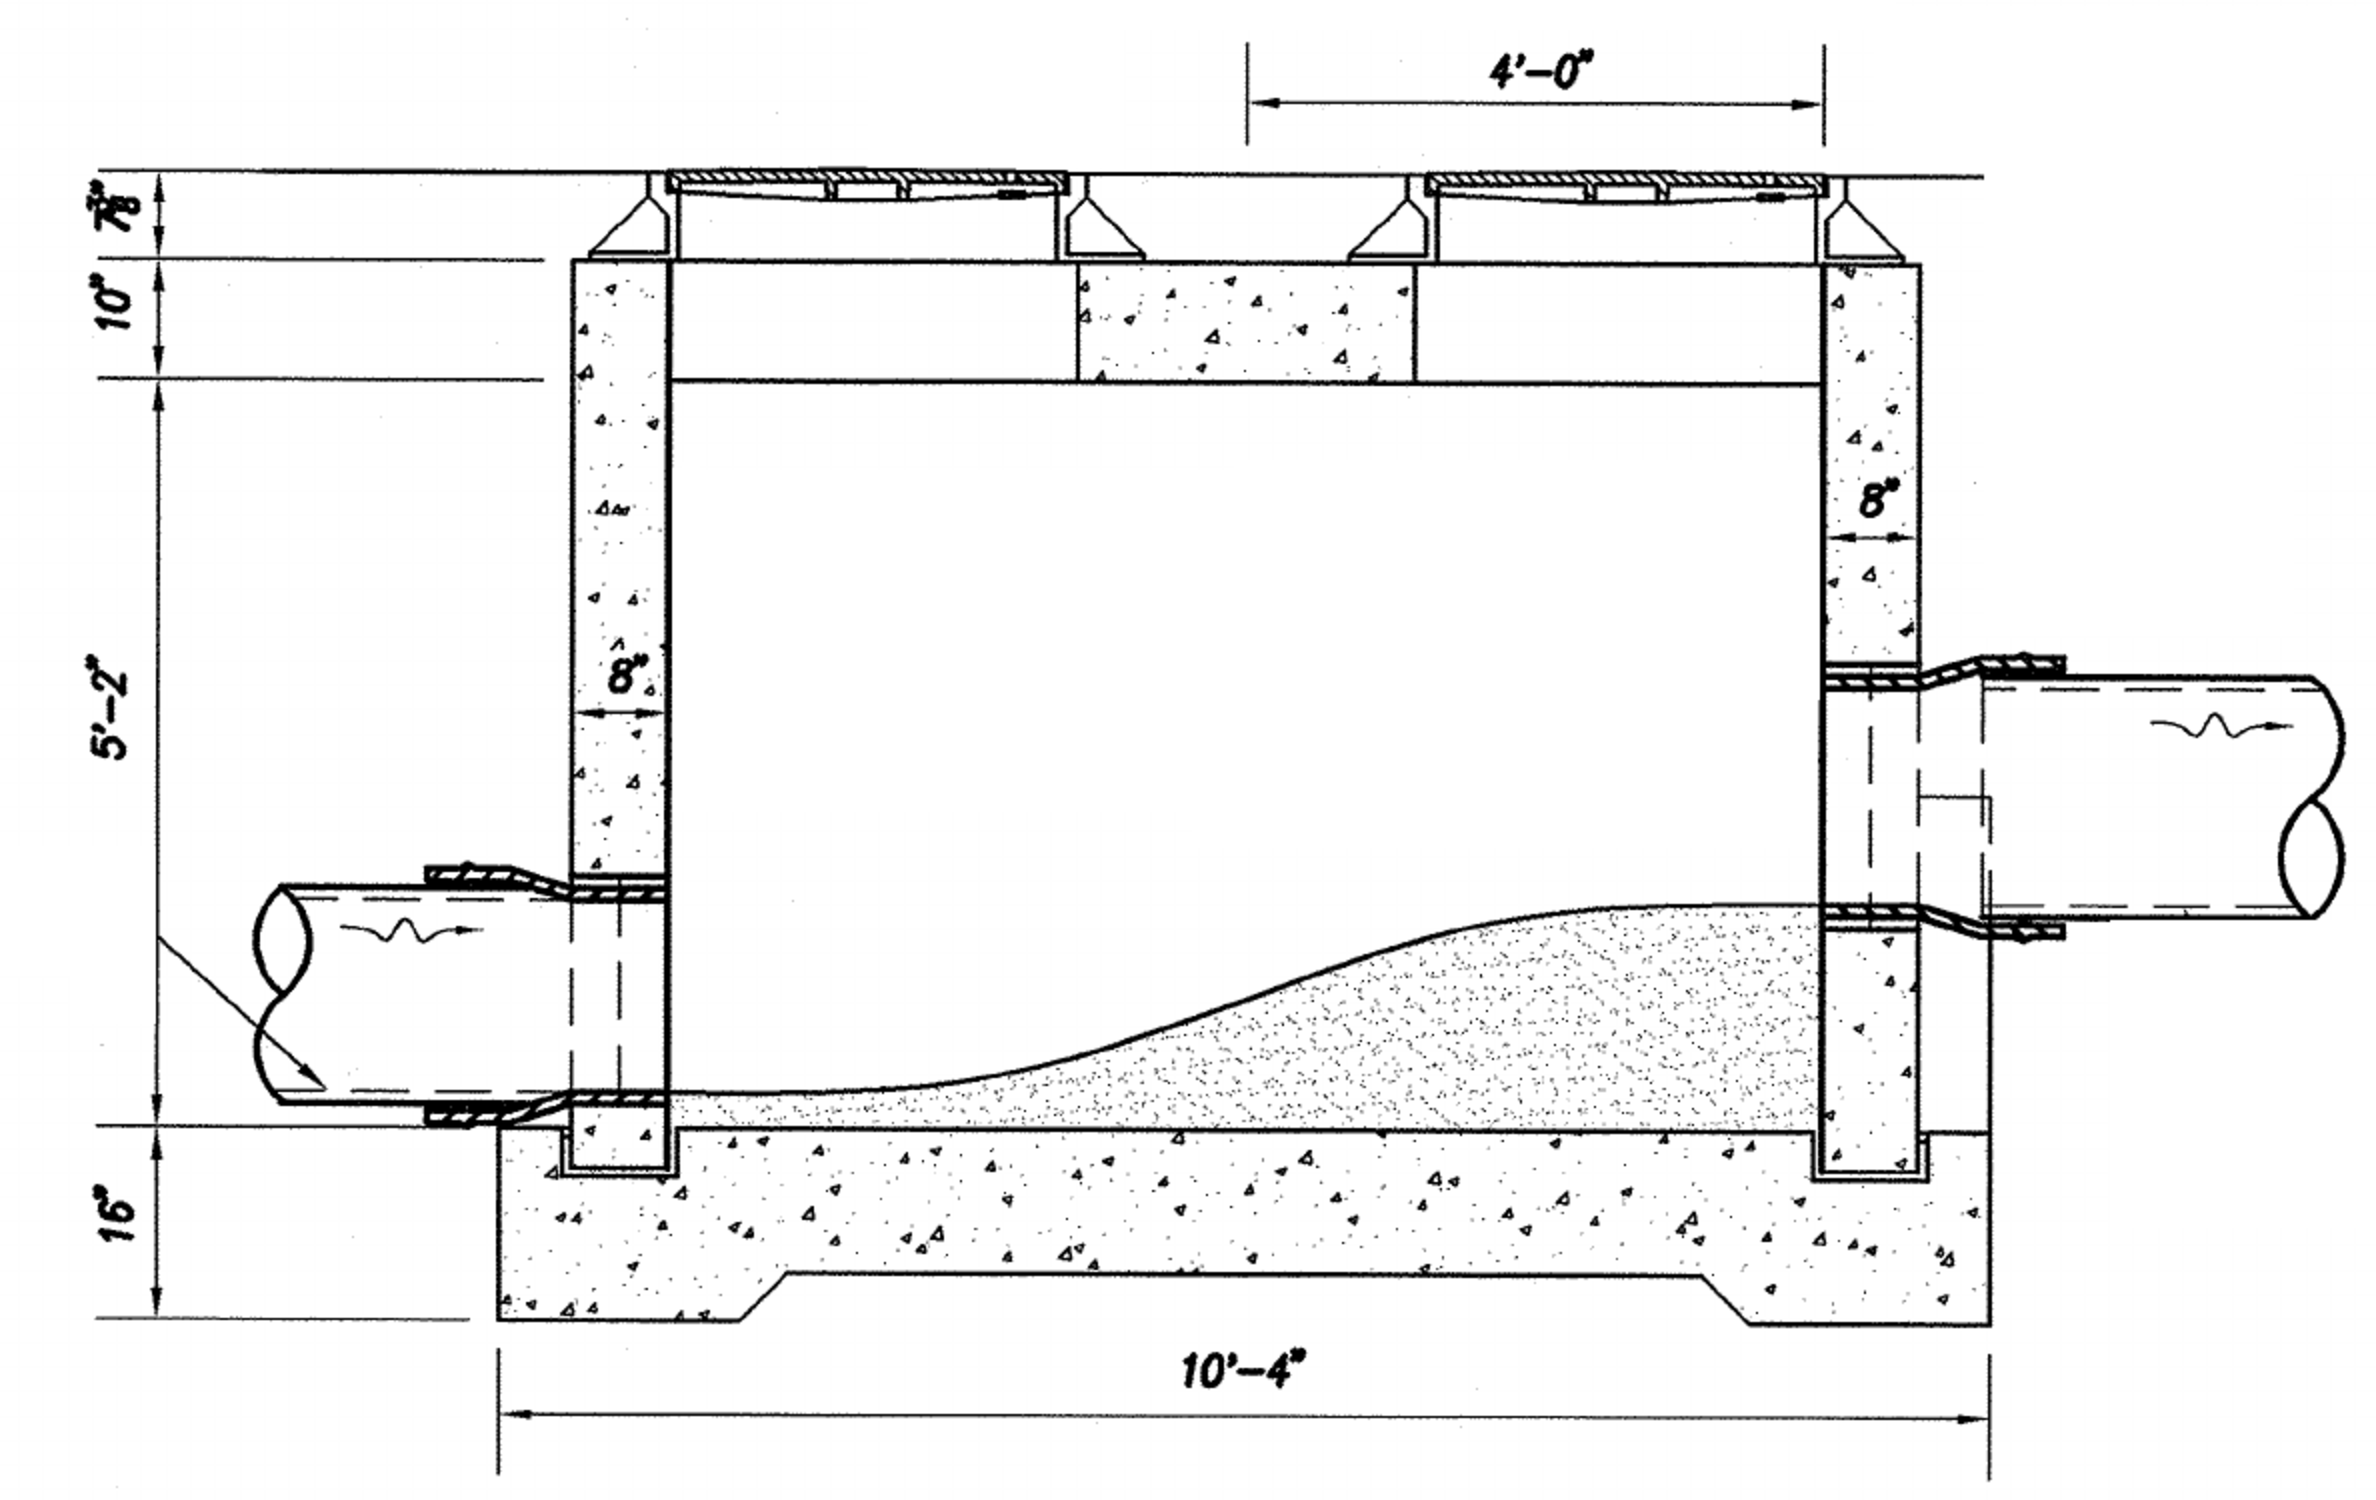
\includegraphics[width=5in]{Figures/Fig01-manhole-simple}
\par\end{centering}
\caption{Section view of a real manhole.}
\label{fig:manhole-section-view}
\end{figure}

\vfill

\newpage\null
\vfill
\begin{figure}[H]
\begin{centering}
(a)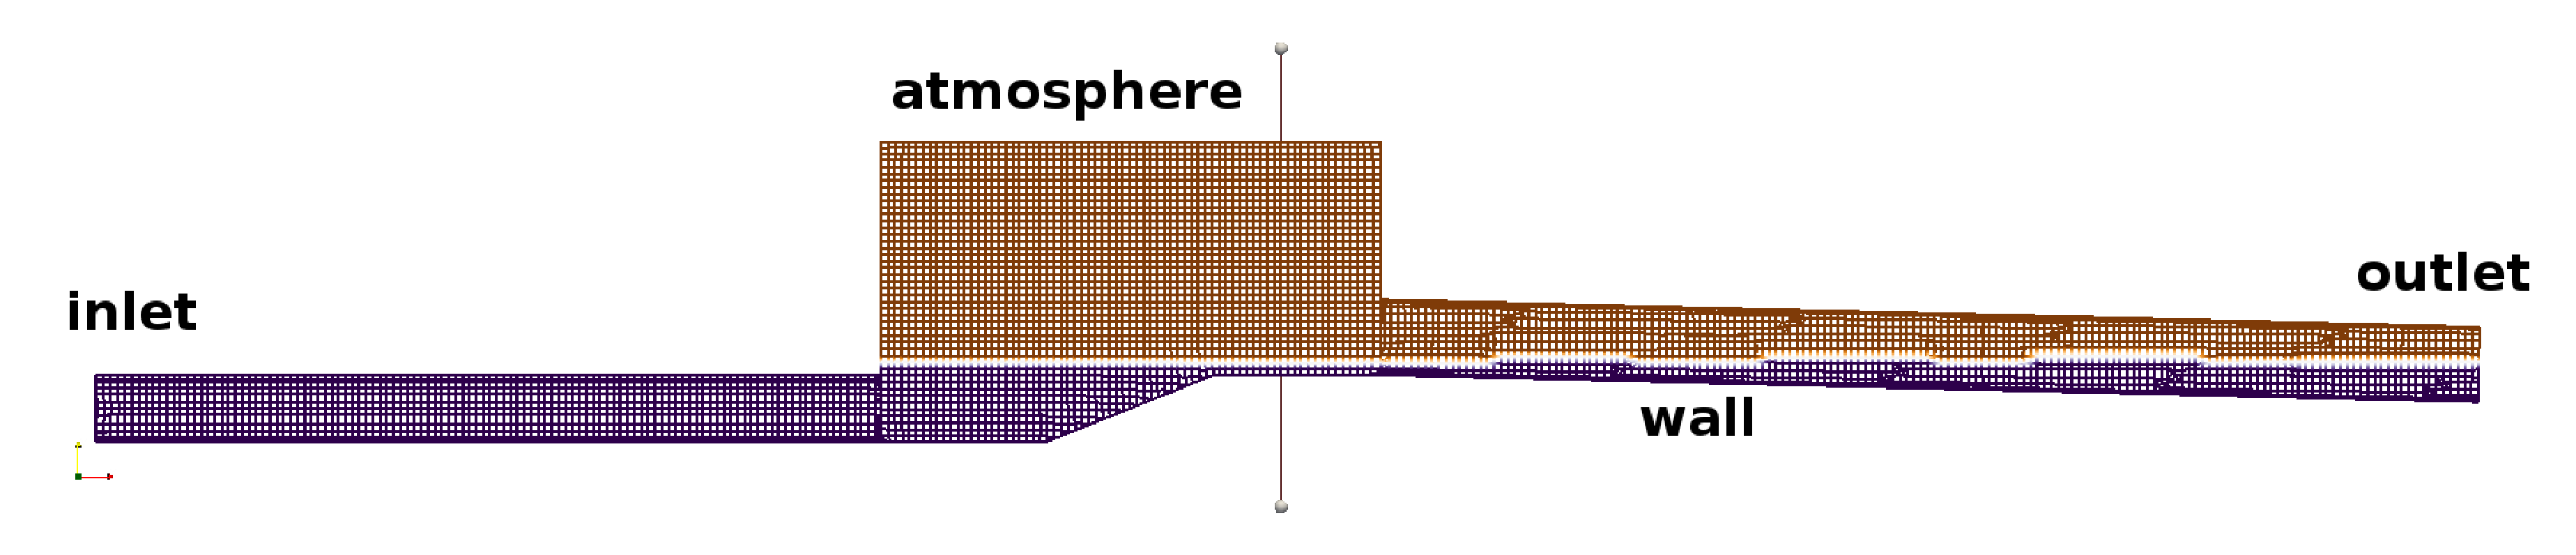
\includegraphics[width=6in]{Figures/Fig02-Mesh-2D-antd}
\par\end{centering}
\begin{centering}
(b)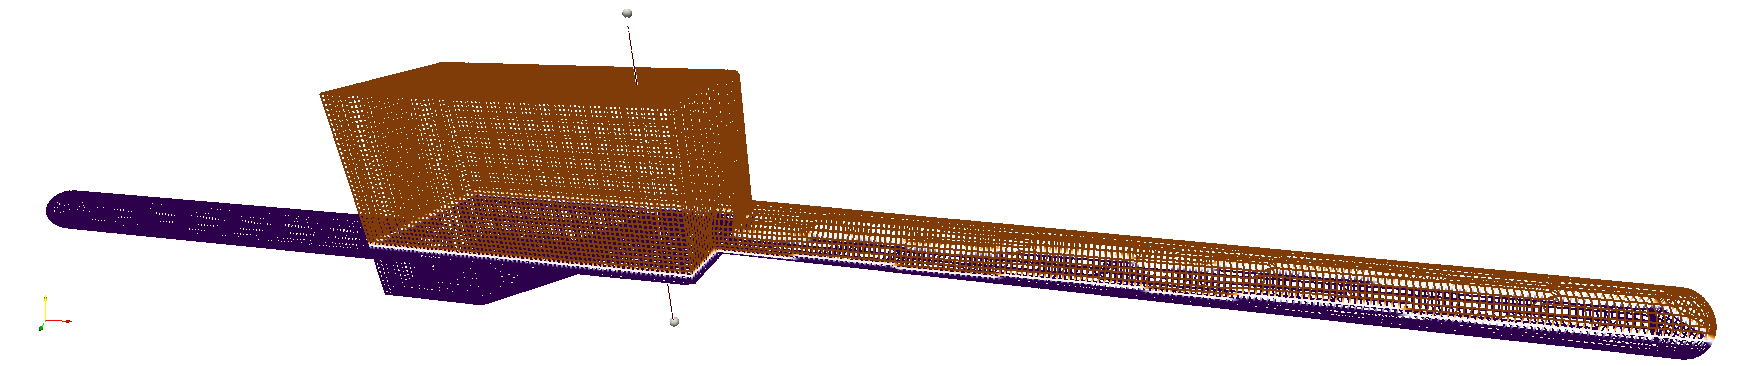
\includegraphics[width=6in]{Figures/Fig02-Mesh-3D}
\par\end{centering}
\caption{Generated mesh structures: (a) 2D and (b) 3D views. The lower purple
and upper brown regions represent water and air phases, respectively.
The vertical line in the $y$-direction near the chamber outlet indicates
a line through which sewage levels are calculated using OpenFOAM simulation
results. In addition, $x$-direction is along the left inlet pipe,
and $z$-direction is out of the $x-y$ plane.}

\label{fig:mesh-struct}
\end{figure}

\vfill


\appendix

\begin{onehalfspace}
\appendix
\end{onehalfspace}

\chapter{Appendix}

\section{Hollow and Filled Unit Stem Generation Using C++ and GNU Make Utility}

\section*{Source code: \texttt{\textmd{gen\_blockMeshToFile-v8.tex}}}

%\lstset{language=C++,basicstyle=\footnotesize}
\begin{lstlisting}[language=C++,numbers=left,basicstyle={\ttfamily},breaklines=true,showspaces=false]
#include <iostream>
#include <fstream>
#include <ctype.h>
#include <stdio.h>
#include <stdlib.h>
#include <unistd.h>
using namespace std;

int main (int argc, char **argv){
  char		cylinderType, comma ; 
                // hollow (h or H) or filled (f or F)
  double	Rinr = 0.5; 
  double	HLCx = 2.0;
  double	HLCy = 2.0;
  int		nGrZ = 5;
  int		Ninr = 8;
  char		idSp,idX, idY;

  std::ifstream infile("blockMesh.param");
  cylinderType= 'F';
  infile    >> Rinr		// >> comma
	    >> HLSq		// >> comma
	    >> FLCz		// >> comma

  std::cout << "infile  = " << "blockMesh.param" << endl;
  std::cout << "Rinr    = " << Rinr << endl;
  std::cout << "HLSq    = " << HLSq << endl;      
 
 /* omitted */  
  
  /* MERGEPATCHPAIRS */
  outfile <<"mergePatchPairs" <<endl;
  outfile <<"("<<endl;
  outfile <<");"<<endl<<endl;
  outfile <<  "// ******************************** //\n"<<endl;

  outfile.close();
  return 0;}
\end{lstlisting}


\paragraph*{Makefile}

\texttt{}
\begin{lstlisting}[language=make,numbers=left,basicstyle={\ttfamily},breaklines=true]
# Makefile 
version=v8
srcroot=gen_blockMeshToFile-$(version)
cxx=g++
# CXX = c++ compiler
# cxx=icpc
#
gbm:
	$(cxx) $(srcroot).cpp -o $(srcroot).x

hollow:
	cp -f blockMesh.param.default blockMesh.param
	sed -i 's/cylinderType/H/' blockMesh.param $(srcroot).x
	cp blockMeshDict_hollow \
		./stem_hollow/stem_hollow/system/blockMeshDict
	cd ./stem_hollow/stem_hollow && blockMesh

filled:
	cp -f blockMesh.param.default blockMesh.param
	sed -i 's/cylinderType/F/' blockMesh.param $(srcroot).x
	cp blockMeshDict_filled \
		./stem_filled/stem_filled/system/blockMeshDict
	cd ./stem_filled/stem_filled && blockMesh
\end{lstlisting}


\section{MATLAB Script to calculate \texttt{alphaU}}

The following script and associated text files were used to produce
\texttt{AlphaU} datasets for each simulation time step. This MATLAB
script was initially used until modifications were made directly in
the OpenFOAM script to automatically calculate \texttt{alphaU}. As
seen in the README.txt section, there are variables within the matlab
script that will need to be changed depending on the OpenFOAM case
and mesh size.

\section*{AlphaU.m}

\begin{lstlisting}[language=Matlab,numbers=left,basicstyle={\ttfamily},breaklines=true,showspaces=true]
% Create Alpha-U Data Set
% Date Created: September 7, 2019
% Last Updated: September 12, 2019
% Created by: Tyler Tsuchida % Document Name: CreateAlphaU.m
% Location: /home/student/Documents/TylerTsuchida/TylerTsuchidaThesis/
% Description: This script is to create a new dataset, alphaU, for every timestep in an openFOAM simulation
%% Read alpha.water and U values from time-step file
%Some lines beyond this point may need revision
num_point_rows=136500; %number of data points within mesh -- given after U or alphawater header
num_boundary_rows=10500; %number of data points at boundaries -- given after boundary conditions are stated at end of U or alphawater
num_headerlines=22; %number of lines from line 1 of code to line before mes data is written
num_boundarylines=5340528; %number of lines from line 1 of code to line before boundary data is written
folder=3; %the next line of code lists all folders in your simulation directory, to skip invisible folders,
folder=1st time step folder on list
timestep=dir('/media/student/Elements/2019-10-25-Coarse/cavity_cFE_coarse0/cavity_cFE_coarse0'); %insert directory with all timesteps here
%Do not need to edit the code beyond this point
% ...
% ...
end
\end{lstlisting}


\section*{\texttt{alphaU} sections}

\subsection*{alphaU\_Header2.txt}

\begin{lstlisting}[language={C++},numbers=left,basicstyle={\ttfamily}]
object alphaU;
}
//*************************************//
dimensions [0 1 -1 0 0 0 0];
internalField nonuniform List<vector>
5340000
(
\end{lstlisting}


\subsection*{alphaU\_Footer1.txt}

\begin{lstlisting}[language={[GNU]C++},numbers=left,breaklines=true]
) ; 
boundaryField 
{  
 DOWN_btm_F00 { type noSlip; } 
 DOWN_btm_H10 { type noSlip; } 
...        
 DOWN_inn_F36 { type noSlip; }
 DOWN_inn_F46 { type noSlip; }
 merged_LEFT_inn_F40 { type flowRateInletVelocity; volumetricFlowRate constant 0.0075; extrapolateProfile false; value uniform (0.3197619 -0 -0); }
 merged_RGHT_btm_F90 { type pressureInletOutletVelocity; value nonuniform List<vector> 10500 ( 
\end{lstlisting}


\subsection*{alphaU\_Footer2.txt}

\begin{lstlisting}[language={C++},numbers=left,breaklines=true]
) ; }
merged_FRNT_inn_F10 { type noSlip; }
merged_FRNT_btm_F00 { type noSlip; }
merged_BACK_inn_F16 { type noSlip; }
merged_BACK_btm_F06 { type noSlip; }
merged_ATOP_inn_F46 { type zeroGradient; }
merged_ATOP_btm_F96 { type zeroGradient; }
}

// *************************************//
\end{lstlisting}


\section*{README.txt}

\begin{lstlisting}[numbers=left,breaklines=true]
Sources for data files:
alphaU_generator.zip
alphaU_generator:
alphaU_Footer1.txt alphaU_Footer2.txt alphaU_Header2.txt calc_alphaU.m README.txt 
All files listed above must be in the directory of all timestep folders for calc_alphaU.m to run properly. 
Enter directory and other information in calc_alphaU.m as needed to match information of the desired run.
\end{lstlisting}


\section{Symmetry Boundary Condition Shear Calculations}

Along with the shear rate calculations presented in the paper, calculations
were also performed on the fine, medium, and coarse meshes using \texttt{cyclic}
boundary conditions. Also, shear rates of the checkerboard were also
calculated as supplementary information.

\begin{table}[H]
\begin{centering}
\begin{tabular}{|c|r|r|r|r|r|r|}
\hline 
Face Name & $\frac{\partial(\alpha U_{x})}{\partial x}$ & $\frac{\partial(\alpha U_{x})}{\partial y}$ & $\frac{\partial(\alpha U_{x})}{\partial z}$ & $\frac{\partial(\alpha U_{y})}{\partial x}$ & $\frac{\partial(\alpha U_{y})}{\partial y}$ & $\frac{\partial(\alpha U_{y})}{\partial z}$\tabularnewline
\hline 
\hline 
DOWN\_Eab\_merged & 2.64E-02 & 6.91E-09 & 3.90E+00 & -- & -- & --\tabularnewline
\hline 
HOLE\_Eab & -1.49E-02 & 1.12E-07 & -6.66E-11 & -- & -- & --\tabularnewline
\hline 
HOLE\_Eab & -- & -- & -- & -1.01E-07 & 1.81E-02 & 8.54E-11\tabularnewline
\hline 
inlet & 1.07E-03 & 0.00E+00 & 0.00E+00 & -- & -- & --\tabularnewline
\hline 
outlet & 1.07E-03 & 1.13E-09 & -2.57E-04 & -- & -- & --\tabularnewline
\hline 
\end{tabular}\caption{Calculations of shear rate {[}1/s{]} using the fine mesh at time =
3.00s with front and back faces (\texttt{cyclic}).}
\par\end{centering}
\label{tbl:fine_mesh_shear_rate-1}
\end{table}


\section{Alternative Canopy Orientations}

The following figures shows alternative configurations of 24 stems
embedded on the bed surface. 

\begin{figure}[H]
\begin{centering}
(a)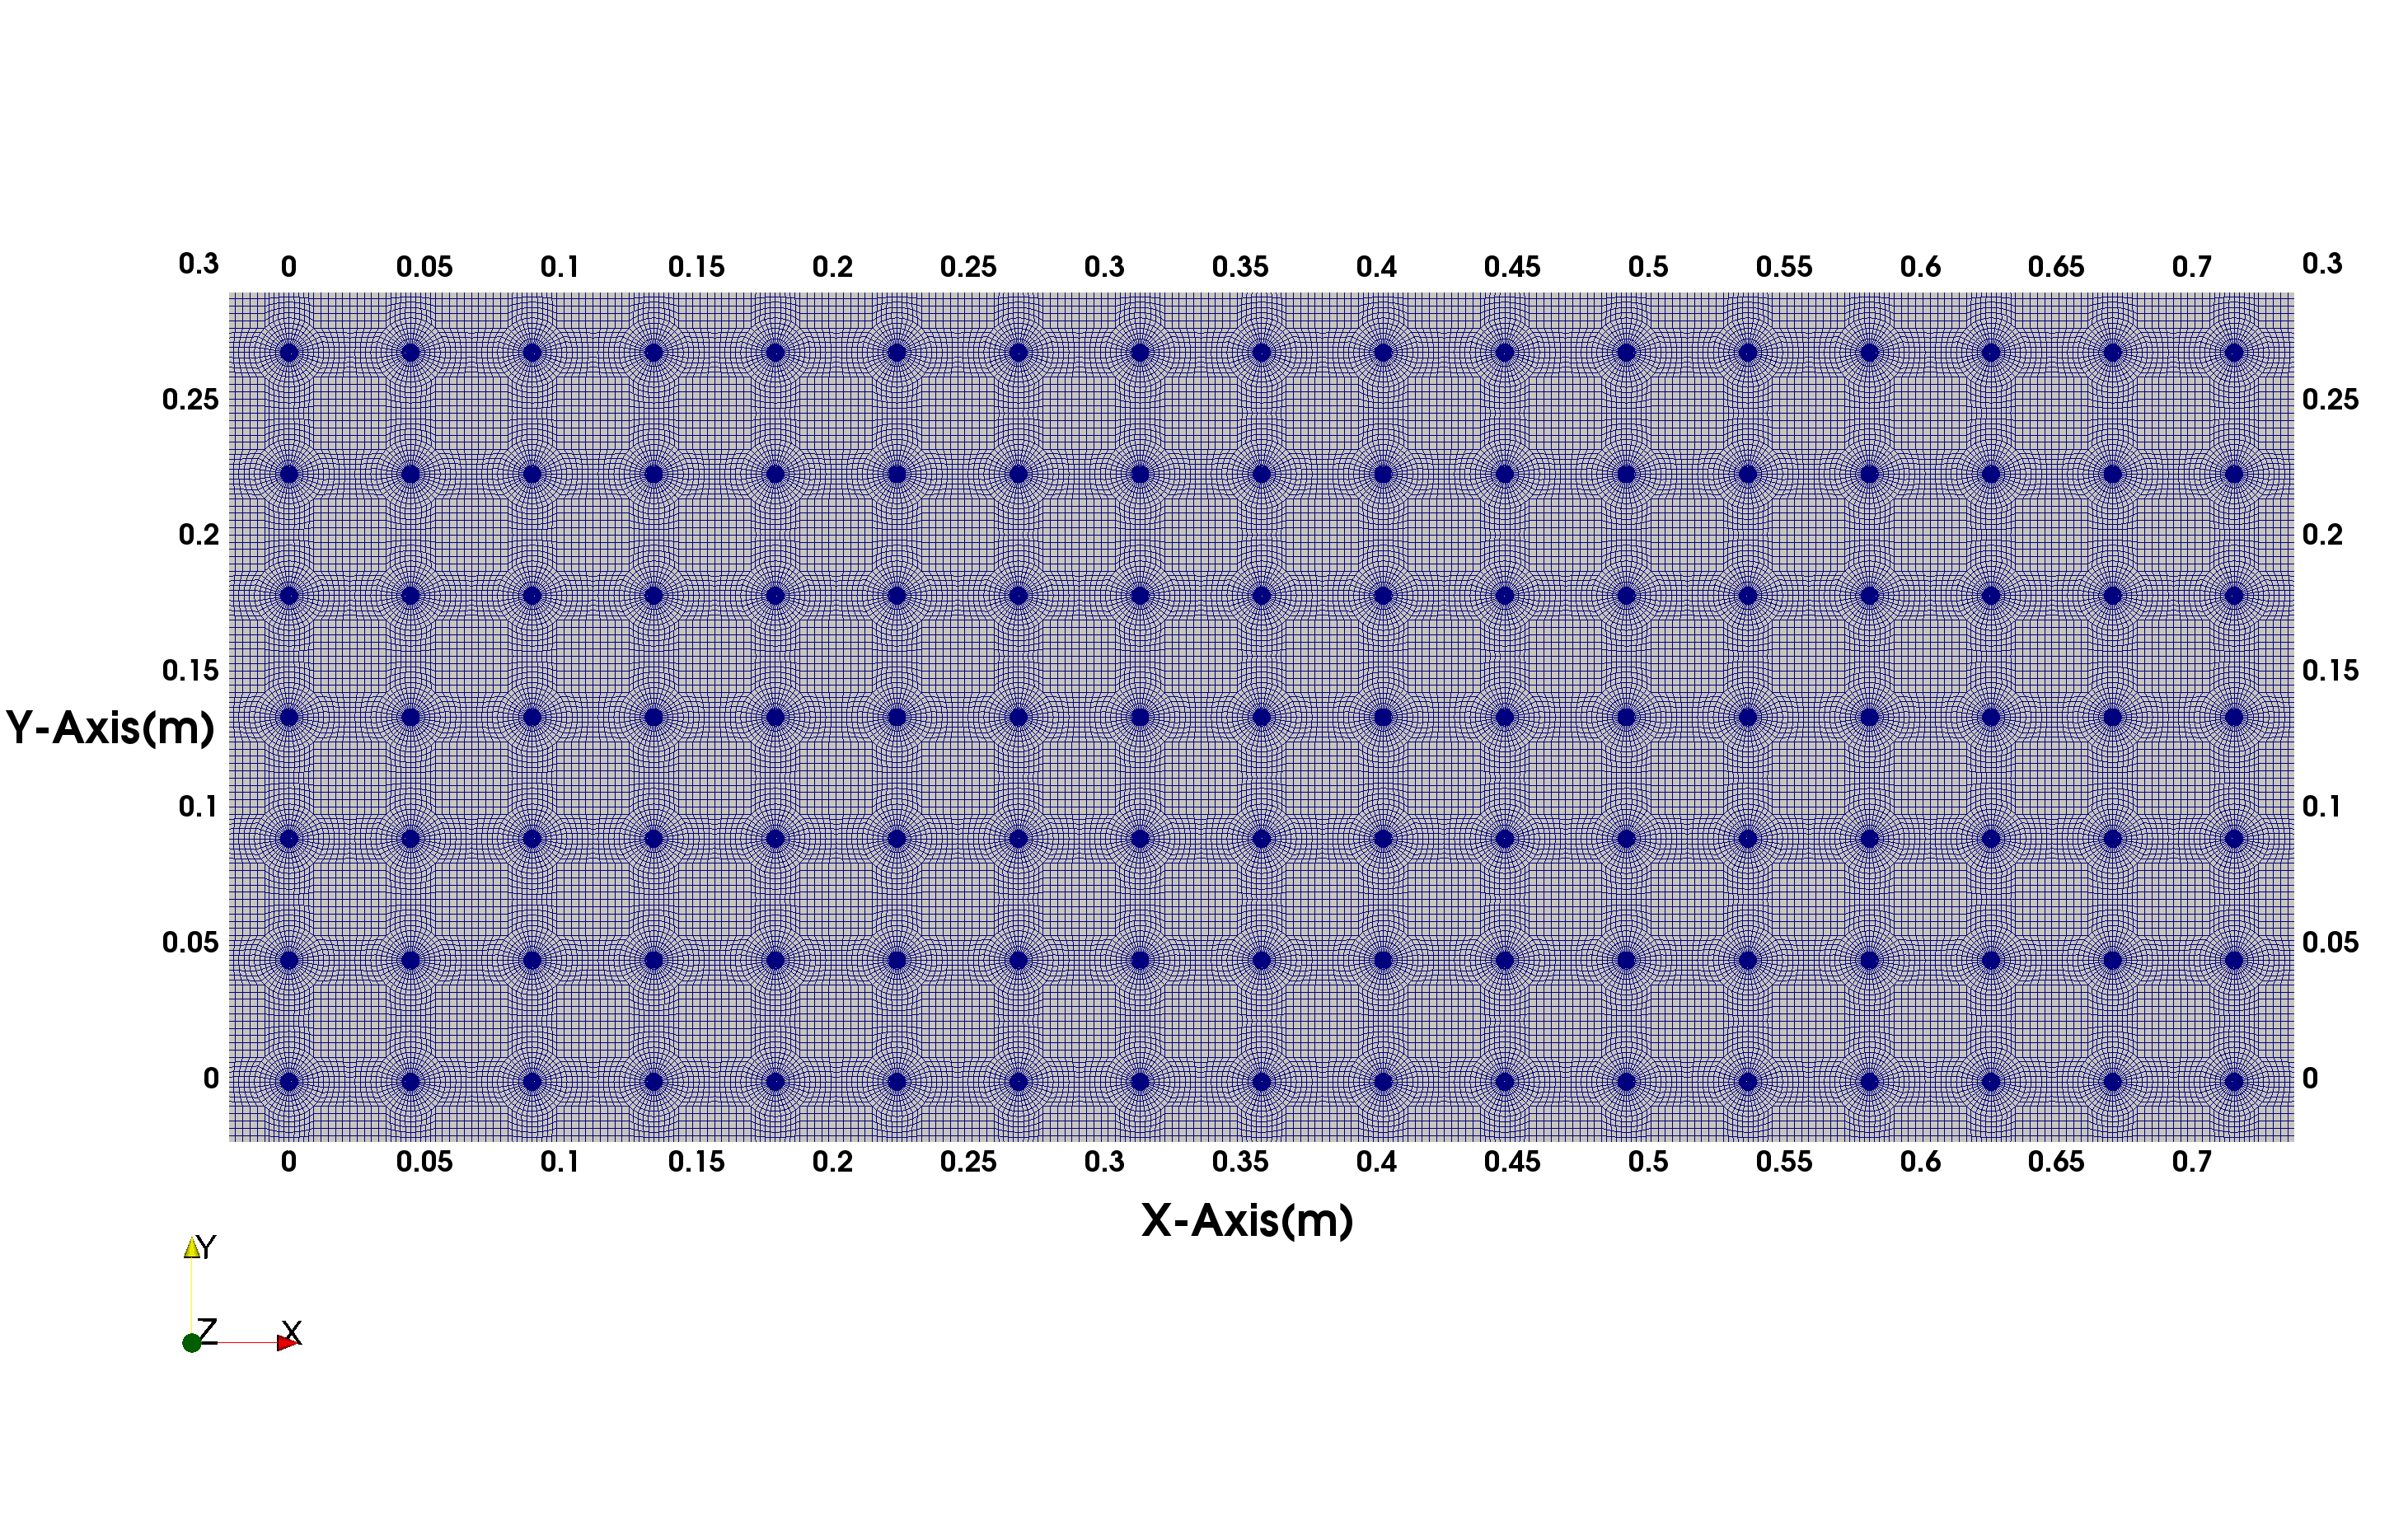
\includegraphics[width=6in]{Figures/0000000_XY}
\par\end{centering}
\begin{centering}
(b)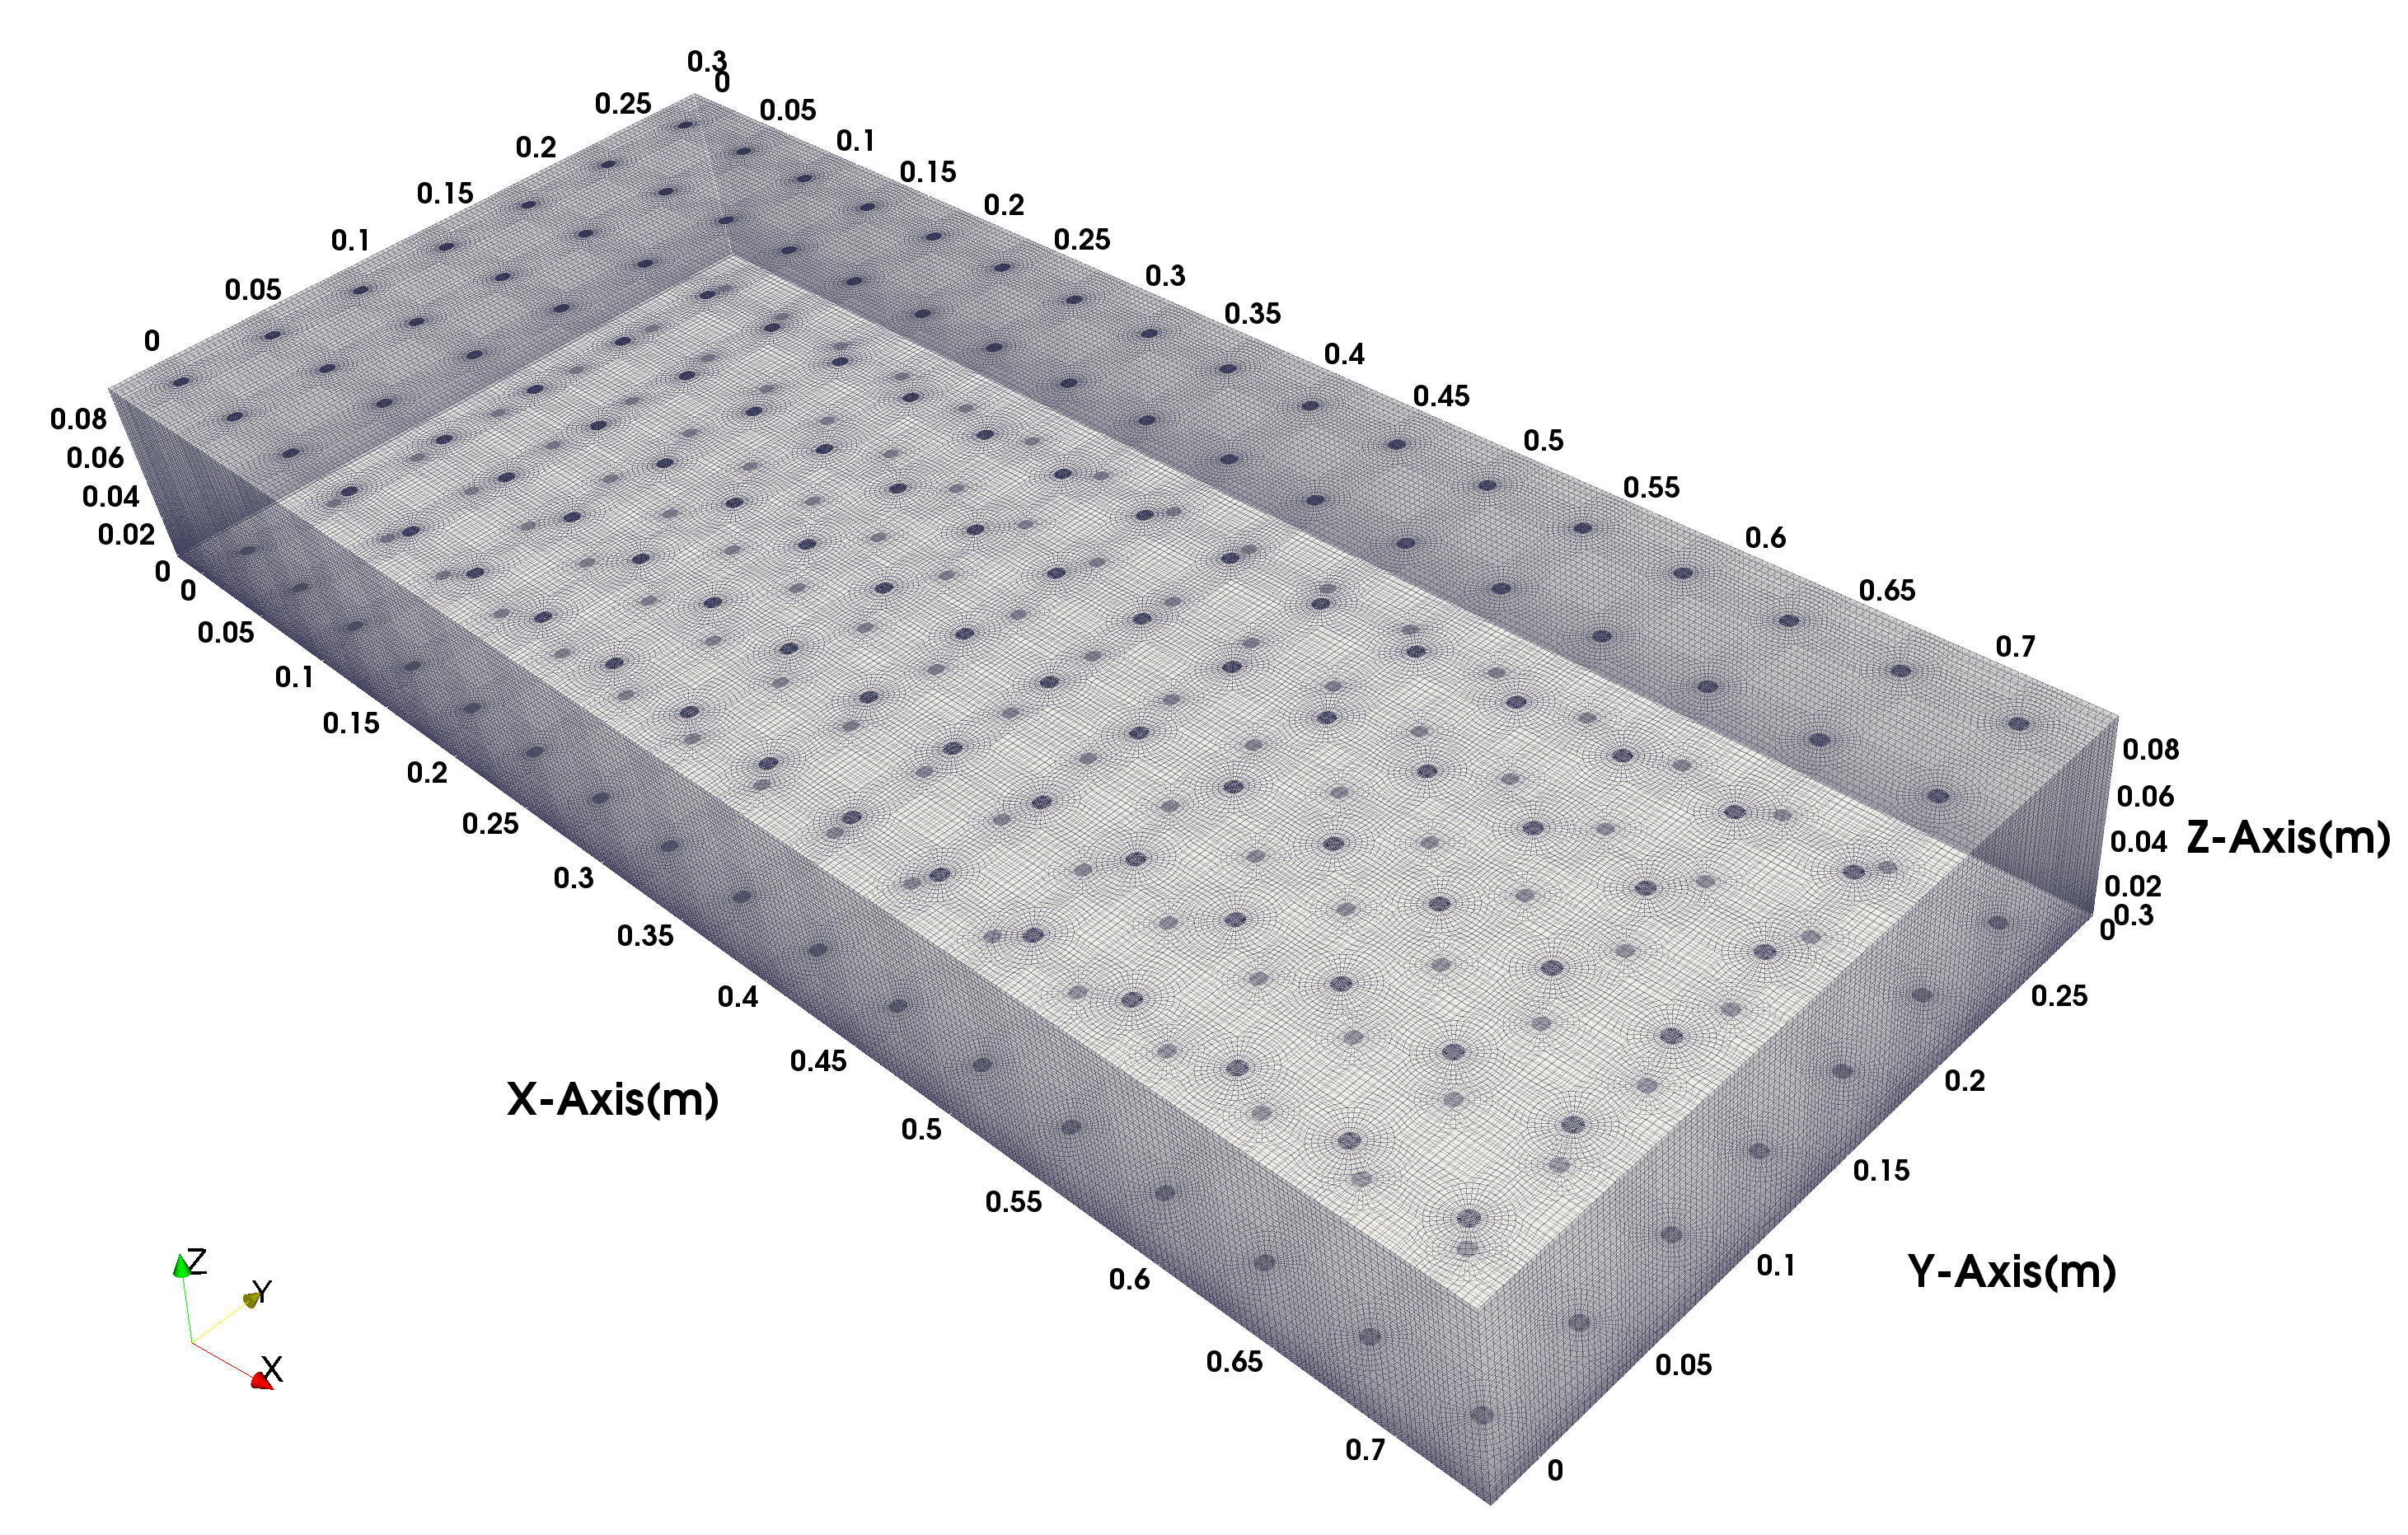
\includegraphics[width=6in]{Figures/0000000_3D}
\par\end{centering}
\caption{0-0-0-0-0-0-0 stem orientation (a)2D and (3) 3D plot.}
\end{figure}

\bibliographystyle{unsrt}
\bibliography{bib/cepl-ref-doi,bib/ShearStressPapers,bib/01_VegetationLayers,bib/02_PracticalImportance,bib/03_DragandRunoff,bib/04_ProblemStatement,bib/AugustCanopyThesis,bib/vegetation_pof,bib/King,bib/LID}

%% Use this for an alphabetically organized bibliography
%\bibliographystyle{plain}
%% Use this for a reference order organized bibliography
%\bibliographystyle{unsrt}
\end{document}
